\section{Platform \& Business Applications}\label{sec:02}  

  The notion of ``platform'' and ``platform-oriented'' software development is nowadays well accepted and in most cases is understood more generically than the capability to operate in a specific operating system.
  Usually, ``platform'' is understood as an execution environment and a set of technologies used for developing software applications for a certain domain.
  Any software application can be based on several platforms, which can be visualised as layers placed on top of each other with the actual application at the very top.
  What is defining for any platform is its unique model that isolates software developers from the details of lower level technologies and platforms.

  \begin{wrapfigure}{r}{55mm}
    \centering    
    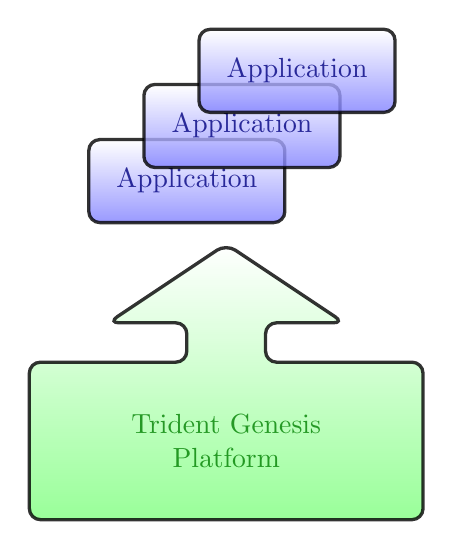
\begin{tikzpicture}[node distance=1cm, auto, opacity=0.8]
      \tikzset{
	  mynode/.style={rectangle,rounded corners,draw=black, top color=white, bottom color=blue!50,very thick, inner sep=1em, minimum size=3em, text centered, text=blue!50!black},
	  platform/.style={rectangle,rounded corners,draw=black, top color=white, bottom color=green!50!white,very thick, inner sep=1em, minimum size=3em, text centered, text=green!50!black}
      }  
      \node at (1, 1) [mynode] (ap1) {Application};
      \node at (1.7, 1.7) [mynode] (ap1) {Application};
      \node at (2.4, 2.4) [mynode] (ap1) {Application};

      \def\platformpath{-- +(5cm,0cm) -- +(5cm,2cm) -- +(3cm,2cm) -- +(3cm,2.5cm) -- +(4cm,2.5cm) -- +(2.5cm,3.5cm) -- +(1cm,2.5cm) -- +(2cm,2.5cm) -- +(2cm,2cm) -- +(0cm,2cm) -- cycle}
      \draw (-1,-3.3) [platform] \platformpath 
	    node [text width=7em, text centered,xshift=2.5cm,yshift=1cm] {Trident Genesis Platform};  
    \end{tikzpicture} 
  \end{wrapfigure}
  
  From this perspective Trident Genesis is not different, providing the necessary abstraction for using lower level technologies without changing the source code of a business application.
  For example, it provides developers with its own model for working with data, which abstracts out the specifics of a particular database.
  This facilitates the use of different databases without modifying the business application source code.
  A small-scale application can happily use H2 or MySQL, while a large-scale application would work with Oracle Database or MS SQL Server.

  At the very beginning the TG platform was targeted inhouse for the purposes of migrating existing business applications away from legacy platfroms and developing new business applications.
  Such a practical-driven approach allowed capturing the existing experience of building business applications in a way that made TG not just a set of reusable components and libraries, but a complete application platform covering every aspect of the application development and deployment life-cycle.
  This in turn positioned TG as a standalone product, which does not include specifics of any particular business application but provides a generic way to build diverse business-oriented information systems.

  The TG platform incorporates a well thought out set of features, which are sufficient for providing solutions to a large variety of business tasks and problems.
  This results in reliable and controlled interoperability between the underlying technologies governed by the platform without the need for introducing external dependencies.
  An excellent example of such interoperability is the TG's \emph{type system}.
  When building applications on top of TG, developers use the provided system of types to uniformly interact with web resources and databases, and implement the business logic and the user interface.
  This removes the need for developers to work on type transformations when implementing the different layers of the information system.
  
  As has been outlined earlier, the majority of software applications are not created from scratch, but enhanced and modified as the business demands.
  It is critical to support the efficient customisation of business applications, particularly by developers who were not involved in the original construction of the system.
  This situation requires such systems to be readily comprehensible, which has been taken into account when designing the TG platform.
  Building applications on top of TG provides a clear separation between the technical and business aspects of the applications, thus providing a much higher level of customisability in order to meet customers' requirements.